\section{Architekturdokumentation}

\subsection{Einführung und Ziele}\label{section-introduction-and-goals}

\subsubsection{Aufgabenstellung}\label{_aufgabenstellung}

\subsubsection{Qualitätsziele}\label{_qualit_tsziele}

\subsubsection{Stakeholder}\label{_stakeholder}

\begin{longtable}[]{@{}lll@{}}
\toprule
\begin{minipage}[b]{0.23\columnwidth}\raggedright\strut
Rolle\strut
\end{minipage} & \begin{minipage}[b]{0.23\columnwidth}\raggedright\strut
Kontakt\strut
\end{minipage} & \begin{minipage}[b]{0.46\columnwidth}\raggedright\strut
Erwartungshaltung\strut
\end{minipage}\tabularnewline
\midrule
\endhead
\begin{minipage}[t]{0.23\columnwidth}\raggedright\strut
\emph{\textless{}Rolle-1\textgreater{}}\strut
\end{minipage} & \begin{minipage}[t]{0.23\columnwidth}\raggedright\strut
\emph{\textless{}Kontakt-1\textgreater{}}\strut
\end{minipage} & \begin{minipage}[t]{0.46\columnwidth}\raggedright\strut
\emph{\textless{}Erwartung-1\textgreater{}}\strut
\end{minipage}\tabularnewline
\begin{minipage}[t]{0.23\columnwidth}\raggedright\strut
\emph{\textless{}Rolle-2\textgreater{}}\strut
\end{minipage} & \begin{minipage}[t]{0.23\columnwidth}\raggedright\strut
\emph{\textless{}Kontakt-2\textgreater{}}\strut
\end{minipage} & \begin{minipage}[t]{0.46\columnwidth}\raggedright\strut
\emph{\textless{}Erwartung-2\textgreater{}}\strut
\end{minipage}\tabularnewline
\bottomrule
\end{longtable}

\subsection{Randbedingungen}\label{section-architecture-constraints}

\subsection{Kontextabgrenzung}\label{section-system-scope-and-context}

\subsubsection{Fachlicher Kontext}\label{_fachlicher_kontext}

\textbf{\textless{}Diagramm und/oder Tabelle\textgreater{}}

\textbf{\textless{}optional: Erläuterung der externen fachlichen
Schnittstellen\textgreater{}}

\subsubsection{Technischer Kontext}\label{_technischer_kontext}

\textbf{\textless{}Diagramm oder Tabelle\textgreater{}}

\textbf{\textless{}optional: Erläuterung der externen technischen
Schnittstellen\textgreater{}}

\textbf{\textless{}Mapping fachliche auf technische
Schnittstellen\textgreater{}}

\subsection{Lösungsstrategie}\label{section-solution-strategy}

\subsection{Bausteinsicht}\label{section-building-block-view}

\subsubsection{Whitebox Gesamtsystem}\label{_whitebox_gesamtsystem}

\emph{\textbf{\textless{}Übersichtsdiagramm\textgreater{}}}

\begin{description}
\item[Begründung]
\emph{\textless{}Erläuternder Text\textgreater{}}
\item[Enthaltene Bausteine]
\emph{\textless{}Beschreibung der enhaltenen Bausteine
(Blackboxen)\textgreater{}}
\item[Wichtige Schnittstellen]
\emph{\textless{}Beschreibung wichtiger Schnittstellen\textgreater{}}
\end{description}

%\subsubsubsection{\textless{}Name Blackbox 1\textgreater{}}\label{__name_blackbox_1}

%\emph{\textless{}Zweck/Verantwortung\textgreater{}}

%\emph{\textless{}Schnittstelle(n)\textgreater{}}

%\emph{\textless{}(Optional) Qualitäts-/Leistungsmerkmale\textgreater{}}

%\emph{\textless{}(Optional) Ablageort/Datei(en)\textgreater{}}

%\emph{\textless{}(Optional) Erfüllte Anforderungen\textgreater{}}

%\emph{\textless{}(optional) Offene Punkte/Probleme/Risiken\textgreater{}}

%\subsubsubsection{\textless{}Name Blackbox 2\textgreater{}}\label{__name_blackbox_2}

%\emph{\textless{}Blackbox-Template\textgreater{}}

%\subsubsubsection{\textless{}Name Blackbox n\textgreater{}}\label{__name_blackbox_n}

%\emph{\textless{}Blackbox-Template\textgreater{}}

%\subsubsubsection{\textless{}Name Schnittstelle 1\textgreater{}}\label{__name_schnittstelle_1}

%\ldots{}

%\subsubsubsection{\textless{}Name Schnittstelle \textgreater{}}\label{__name_schnittstelle_m}

%\subsubsection{Ebene 2}\label{_ebene_2}

%\subsubsubsection{\texorpdfstring{Whitebox \emph{\textless{}Baustein 1\textgreater{}}}{Whitebox \textless{}Baustein 1\textgreater{}}}\label{_whitebox_emphasis_baustein_1_emphasis}

%\emph{\textless{}Whitebox-Template\textgreater{}}

%\subsubsubsection{\texorpdfstring{Whitebox \emph{\textless{}Baustein 2\textgreater{}}}{Whitebox \textless{}Baustein 2\textgreater{}}}\label{_whitebox_emphasis_baustein_2_emphasis}

%\emph{\textless{}Whitebox-Template\textgreater{}}

%\ldots{}

%\subsubsubsection{\texorpdfstring{Whitebox \emph{\textless{}Baustein m\textgreater{}}}{Whitebox \textless{}Baustein m\textgreater{}}}\label{_whitebox_emphasis_baustein_m_emphasis}

%\emph{\textless{}Whitebox-Template\textgreater{}}

%\subsubsection{Ebene 3}\label{_ebene_3}

%\subsubsubsection{Whitebox \textless{}\_Baustein x.1\_\textgreater{}}\label{_whitebox_baustein_x_1}

%\emph{\textless{}Whitebox-Template\textgreater{}}

%\subsubsubsection{Whitebox \textless{}\_Baustein x.2\_\textgreater{}}\label{_whitebox_baustein_x_2}

%\emph{\textless{}Whitebox-Template\textgreater{}}

%\subsubsubsection{Whitebox \textless{}\_Baustein y.1\_\textgreater{}}\label{_whitebox_baustein_y_1}

%\emph{\textless{}Whitebox-Template\textgreater{}}

\subsection{Laufzeitsicht}\label{section-runtime-view}

\subsubsection{\texorpdfstring{\emph{\textless{}Bezeichnung
Laufzeitszenario
1\textgreater{}}}{\textless{}Bezeichnung Laufzeitszenario 1\textgreater{}}}\label{__emphasis_bezeichnung_laufzeitszenario_1_emphasis}

\begin{itemize}
\item
  \textless{}hier Laufzeitdiagramm oder Ablaufbeschreibung
  einfügen\textgreater{}
\item
  \textless{}hier Besonderheiten bei dem Zusammenspiel der Bausteine in
  diesem Szenario erläutern\textgreater{}
\end{itemize}

\subsubsection{\texorpdfstring{\emph{\textless{}Bezeichnung
Laufzeitszenario
2\textgreater{}}}{\textless{}Bezeichnung Laufzeitszenario 2\textgreater{}}}\label{__emphasis_bezeichnung_laufzeitszenario_2_emphasis}

\ldots{}

\subsubsection{\texorpdfstring{\emph{\textless{}Bezeichnung
Laufzeitszenario
n\textgreater{}}}{\textless{}Bezeichnung Laufzeitszenario n\textgreater{}}}\label{__emphasis_bezeichnung_laufzeitszenario_n_emphasis}

\ldots{}

\subsection{Verteilungssicht}\label{section-deployment-view}

\subsubsection{Infrastruktur Ebene 1}\label{_infrastruktur_ebene_1}

\emph{\textbf{\textless{}Übersichtsdiagramm\textgreater{}}}

\begin{description}
\item[Begründung]
\emph{\textless{}Erläuternder Text\textgreater{}}
\item[Qualitäts- und/oder Leistungsmerkmale]
\emph{\textless{}Erläuternder Text\textgreater{}}
\item[Zuordnung von Bausteinen zu Infrastruktur]
\emph{\textless{}Beschreibung der Zuordnung\textgreater{}}
\end{description}

\subsubsection{Infrastruktur Ebene 2}
\label{_infrastruktur_ebene_2}

\begin{figure}[h]
    \centering
    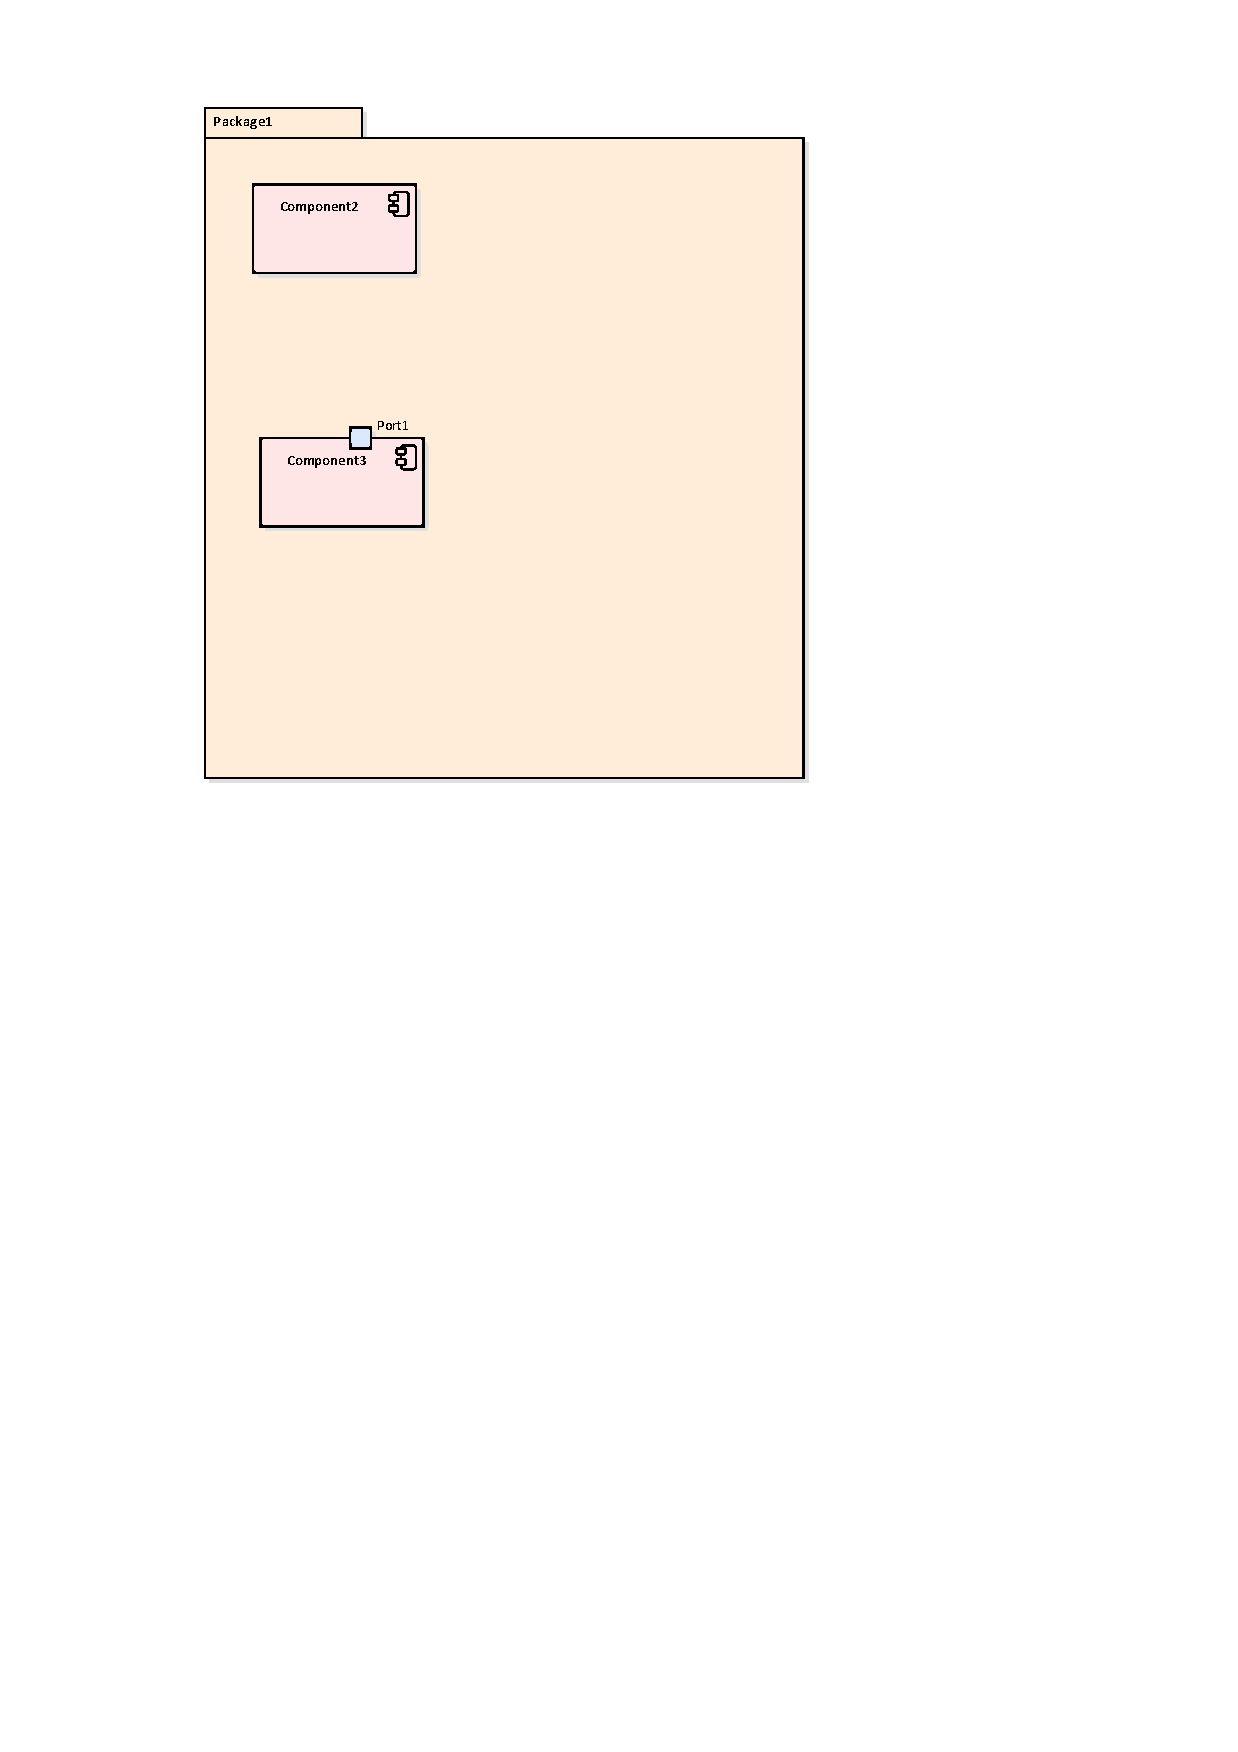
\includegraphics[width=1\textwidth]{dd.pdf}
    \caption{Schematical view of Spearman's theory.}
\end{figure}



%\subsubsubsection{\texorpdfstring{\emph{\textless{}Infrastrukturelement 1\textgreater{}}}{\textless{}Infrastrukturelement 1\textgreater{}}}\label{__emphasis_infrastrukturelement_1_emphasis}

%\emph{\textless{}Diagramm + Erläuterungen\textgreater{}}

%\subsubsubsection{\texorpdfstring{\emph{\textless{}Infrastrukturelement 2\textgreater{}}}{\textless{}Infrastrukturelement 2\textgreater{}}}\label{__emphasis_infrastrukturelement_2_emphasis}

%\emph{\textless{}Diagramm + Erläuterungen\textgreater{}}

%\ldots{}

%\subsubsubsection{\texorpdfstring{\emph{\textless{}Infrastrukturelement n\textgreater{}}}{\textless{}Infrastrukturelement n\textgreater{}}}\label{__emphasis_infrastrukturelement_n_emphasis}

%\emph{\textless{}Diagramm + Erläuterungen\textgreater{}}

\subsection{Querschnittliche Konzepte}\label{section-concepts}

\subsubsection{\texorpdfstring{\emph{\textless{}Konzept
1\textgreater{}}}{\textless{}Konzept 1\textgreater{}}}\label{__emphasis_konzept_1_emphasis}

\emph{\textless{}Erklärung\textgreater{}}

\subsubsection{\texorpdfstring{\emph{\textless{}Konzept
2\textgreater{}}}{\textless{}Konzept 2\textgreater{}}}\label{__emphasis_konzept_2_emphasis}

\emph{\textless{}Erklärung\textgreater{}}

\ldots{}

\subsubsection{\texorpdfstring{\emph{\textless{}Konzept
n\textgreater{}}}{\textless{}Konzept n\textgreater{}}}\label{__emphasis_konzept_n_emphasis}

\emph{\textless{}Erklärung\textgreater{}}

\subsection{Entwurfsentscheidungen}\label{section-design-decisions}

\subsection{Qualitätsanforderungen}\label{section-quality-scenarios}

\subsubsection{Qualitätsbaum}\label{_qualit_tsbaum}

\subsubsection{Qualitätsszenarien}\label{_qualit_tsszenarien}

\subsection{Risiken und technische Schulden}\label{section-technical-risks}

\subsection{Glossar}\label{section-glossary}

\begin{longtable}[]{@{}ll@{}}
\toprule
\begin{minipage}[b]{0.31\columnwidth}\raggedright\strut
Begriff\strut
\end{minipage} & \begin{minipage}[b]{0.63\columnwidth}\raggedright\strut
Definition\strut
\end{minipage}\tabularnewline
\midrule
\endhead
\begin{minipage}[t]{0.31\columnwidth}\raggedright\strut
\emph{\textless{}Begriff-1\textgreater{}}\strut
\end{minipage} & \begin{minipage}[t]{0.63\columnwidth}\raggedright\strut
\emph{\textless{}Definition-1\textgreater{}}\strut
\end{minipage}\tabularnewline
\begin{minipage}[t]{0.31\columnwidth}\raggedright\strut
\emph{\textless{}Begriff-2}\strut
\end{minipage} & \begin{minipage}[t]{0.63\columnwidth}\raggedright\strut
\emph{\textless{}Definition-2\textgreater{}}\strut
\end{minipage}\tabularnewline
\bottomrule
\end{longtable}
